%----------------------------------------------------------------------------------------
%	PACKAGES AND OTHER DOCUMENT CONFIGURATIONS
%----------------------------------------------------------------------------------------
\documentclass[12pt]{article}
\usepackage{graphicx}
\usepackage{amsmath,amsfonts,stmaryrd,amssymb} % Math packages
\usepackage{bm}
\usepackage{steinmetz}
\usepackage{enumitem}
\graphicspath{{images/}}
\usepackage{float}
\usepackage{cancel}
\usepackage{hyperref}
\hypersetup{
	colorlinks=true,
	linkcolor=blue,
	filecolor=magenta,      
	urlcolor=cyan,
	pdftitle={Overleaf Example},
	pdfpagemode=FullScreen,
}
\urlstyle{same}
\usepackage{mathtools}
\usepackage{fancyhdr}
\usepackage{xcolor}
\usepackage[american,RPvoltages]{circuiTikz}
\usepackage{tikz, tikz-cd}
\usepackage{pgfplots}
\usepackage{siunitx}
\usetikzlibrary{spy,shapes,arrows, arrows.meta, bending, decorations.markings}
\pgfplotsset{width=10cm,compat=1.18}
\usepackage{lmodern} % package for changing font size
\usepackage{lastpage}
\renewcommand{\figurename}{Figura}
\usepackage{tcolorbox}
\usepackage{lipsum}
%\usepackage{enumerate} % Custom item numbers for enumerations
\usepackage[ruled]{algorithm2e} % Algorithms
\usepackage[framemethod=tikz]{mdframed} % Allows defining custom boxed/framed environments
\usepackage{listings} % File listings, with syntax highlighting
%\lstset{basicstyle=\ttfamily,} % Typeset listings in monospace font
\usepackage{lipsum}
\tcbuselibrary{listings,theorems,skins,vignette,raster,breakable,magazine,poster,fitting,hooks}
\usepackage[T1]{fontenc}
\usepackage{tgbonum}
 \fontfamily{garamond}
\definecolor{myblue}{RGB}{24, 51, 73}
%----------------------------------------------------------------------------------------
%	DOCUMENT MARGINS
%----------------------------------------------------------------------------------------

\usepackage{geometry} % Required for adjusting page dimensions and margins
\geometry{
	paper=a4paper, % Paper size, change to letterpaper for US letter size
	top=2.5cm, % Top margin
	bottom=3cm, % Bottom margin
	left=2cm, % Left margin
	right=2.5cm, % Right margin
	headheight=14pt, % Header height
	footskip=1.5cm, % Space from the bottom margin to the baseline of the footer
	headsep=1.2cm, % Space from the top margin to the baseline of the header
	%showframe, % Uncomment to show how the type block is set on the page
}

%----------------------------------------------------------------------------------------
%	FONTS
%----------------------------------------------------------------------------------------

\usepackage[utf8]{inputenc} % Required for inputting international characters
\usepackage[T1]{fontenc} % Output font encoding for international characters
\usepackage{XCharter} % Use the XCharter fonts
\usepackage{tgbonum}
\ctikzset{bipoles/thickness=1.2}
\makeatletter
\pgfcircdeclarebipole{}{\ctikzvalof{bipoles/vsourcesin/height}}{sVpm}{\ctikzvalof{bipoles/vsourcesin/height}}{\ctikzvalof{bipoles/vsourcesin/width}}{
	
	\pgfsetlinewidth{\pgfkeysvalueof{/tikz/circuitikz/bipoles/thickness}\pgfstartlinewidth}
	\pgfpathellipse{\pgfpointorigin}{\pgfpoint{0}{\pgf@circ@res@up}}{\pgfpoint{\pgf@circ@res@left}{0}}
	\pgfusepath{draw}     
	\pgftext[bottom,rotate=90,y=\ctikzvalof{bipoles/vsourceam/margin}\pgf@circ@res@down]{\scriptsize$-$}
	\pgftext[top,rotate=90,y=\ctikzvalof{bipoles/vsourceam/margin}\pgf@circ@res@up]{\scriptsize$+$}
	
	\pgf@circ@res@up = .35\pgf@circ@res@up
	\pgfscope
	\pgftransformrotate{90}
	\pgfpathmoveto{\pgfpoint{-\pgf@circ@res@up}{0cm}}
	\pgfpathsine{\pgfpoint{.5\pgf@circ@res@up}{.4\pgf@circ@res@up}}
	\pgfpathcosine{\pgfpoint{.5\pgf@circ@res@up}{-.4\pgf@circ@res@up}}
	\pgfpathsine{\pgfpoint{.5\pgf@circ@res@up}{-.4\pgf@circ@res@up}}
	\pgfpathcosine{\pgfpoint{.5\pgf@circ@res@up}{.4\pgf@circ@res@up}}
	\pgfusepath{draw}
	\endpgfscope
}
\def\pgf@circ@sVpm@path#1{\pgf@circ@bipole@path{sVpm}{#1}}
\compattikzset{sinusoidal voltage source pm/.style = {\circuitikzbasekey, /tikz/to path=\pgf@circ@sVpm@path, \circuitikzbasekey/bipole/is voltage=true, \circuitikzbasekey/bipole/is voltageoutsideofsymbol=true, v=#1 }}
\compattikzset{sVpm/.style = {\comnpatname sinusoidal voltage source pm = #1}}

\pgfcircdeclarebipole{}{\ctikzvalof{bipoles/vsourcesin/height}}{sVpmh}{\ctikzvalof{bipoles/vsourcesin/height}}{\ctikzvalof{bipoles/vsourcesin/width}}{
	
	\pgfsetlinewidth{\pgfkeysvalueof{/tikz/circuitikz/bipoles/thickness}\pgfstartlinewidth}
	\pgfpathellipse{\pgfpointorigin}{\pgfpoint{0}{\pgf@circ@res@up}}{\pgfpoint{\pgf@circ@res@left}{0}}
	\pgfusepath{draw}     
	\pgftext[center,x=0.2\pgf@circ@res@down-\ctikzvalof{bipoles/vsourceam/margin}\pgf@circ@res@down]{\scriptsize$-$}
	\pgftext[top,rotate=90,y=\ctikzvalof{bipoles/vsourceam/margin}\pgf@circ@res@up]{\scriptsize$+$}
	
	\pgf@circ@res@up = .35\pgf@circ@res@up
	\pgfscope
	\pgftransformrotate{90}
	\pgfpathmoveto{\pgfpoint{-\pgf@circ@res@up}{0cm}}
	\pgfpathsine{\pgfpoint{.5\pgf@circ@res@up}{.4\pgf@circ@res@up}}
	\pgfpathcosine{\pgfpoint{.5\pgf@circ@res@up}{-.4\pgf@circ@res@up}}
	\pgfpathsine{\pgfpoint{.5\pgf@circ@res@up}{-.4\pgf@circ@res@up}}
	\pgfpathcosine{\pgfpoint{.5\pgf@circ@res@up}{.4\pgf@circ@res@up}}
	\pgfusepath{draw}
	\endpgfscope
}
\def\pgf@circ@sVpmh@path#1{\pgf@circ@bipole@path{sVpmh}{#1}}
\compattikzset{sinusoidal voltage source pmh/.style = {\circuitikzbasekey, /tikz/to path=\pgf@circ@sVpmh@path, \circuitikzbasekey/bipole/is voltage=true, \circuitikzbasekey/bipole/is voltageoutsideofsymbol=true, v=#1 }}
\compattikzset{sVpmh/.style = {\comnpatname sinusoidal voltage source pmh = #1}}
\makeatother


%----------------------------------------------------------------------------------------
%	BEGIN DOCUMENT
%----------------------------------------------------------------------------------------

\begin{document}
	%\thispagestyle{empty}
	\begin{tikzpicture}[remember picture, overlay]
		\node[anchor=north west, inner sep=0pt] at (current page.north west) {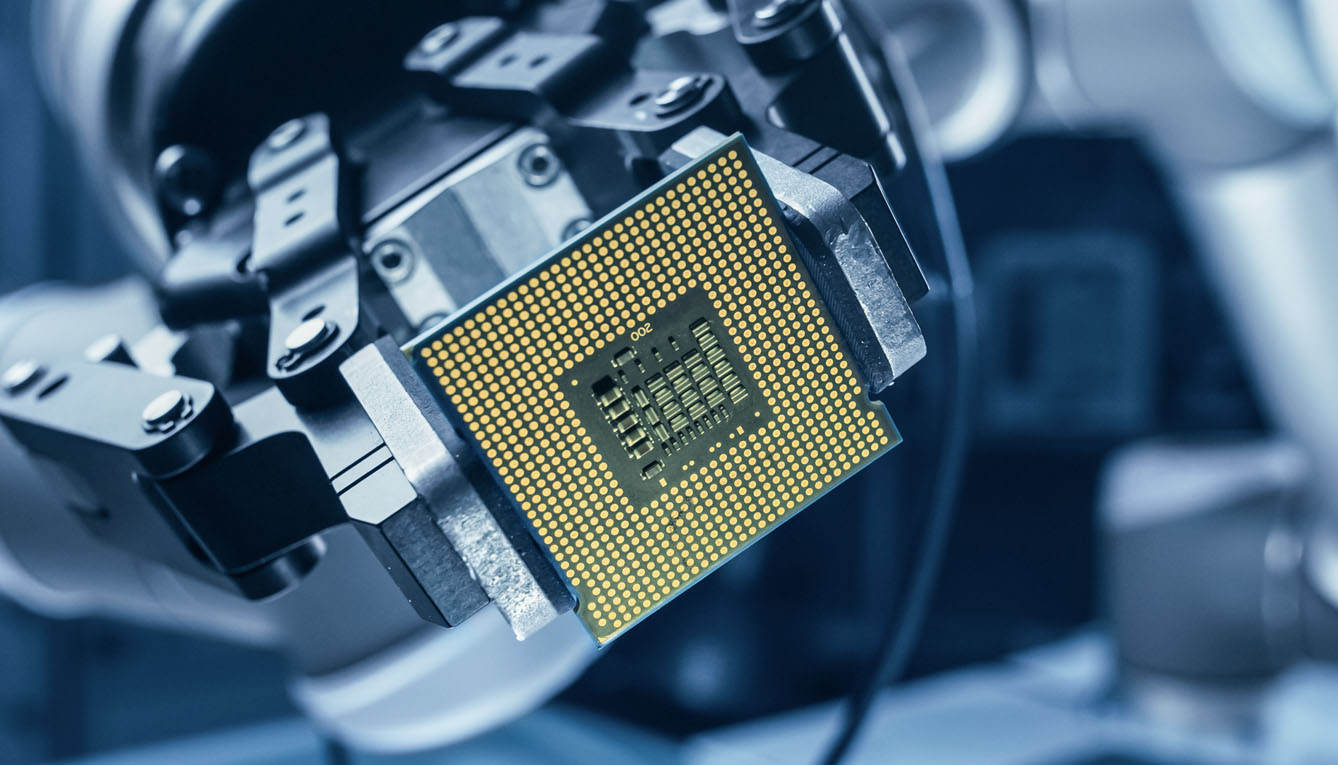
\includegraphics[width=\paperwidth, height=.5\paperheight]{picture1}};
	\end{tikzpicture}

	\vspace{13cm}
	\noindent \textcolor{myblue}{\fontsize{40pt}{40pt}\selectfont \textbf{Ecuaciones simultáneas con OpAmps}}\\\\
	{\fontsize{18pt}{18pt}\selectfont Noviembre, 2023} 
	
	\newpage
	\section*{Introducción}
	La mayoría de los sistemas portables usan una batería, la creciente popularidad de los equipos portables resulta en un incremento del uso de fuentes de alimentación unipolares. El diseño con amplificadores operacionales que usan fuentes duales o bipolares es en parte sencillo porque las entradas y salidas del amplificador operacional están referenciadas a una toma central de ambas fuentes de alimentación normalmente conectada a tierra. En la mayoría de las aplicaciones con fuentes duales, la fuente de señal conectada en la entrada del amplificador operacional está referenciada a tierra, por lo tanto, con una entrada del amplificador operacional conectada a tierra como se muestra en la figura 1, el voltaje en modo común y los problemas de polarización de voltajes son despreciables.
	
	\begin{figure}[H]
		\centering	
		\begin{tikzpicture}[]
			\ctikzset{%
				 monopoles/vcc/arrow={Triangle[width=0.8*\scaledwidth, length=\scaledwidth]},
				 monopoles/vee/arrow={Triangle[width=6pt, length=8pt]},
				 }
			\draw (0,0) to[short] (0,0) coordinate(TW);
			\draw (TW.east) -- ++(1,0) node[op amp, anchor=-](A1){};
			\draw (A1.up) -- ++(0, 0.3) node[vcc]{+V};
			\draw (A1.down) -- ++(0,-0.3) node[vee]{-V};
			\draw (A1.+) -- ++(-1,0) to[short] ++(0,-0.5) node[ground]{};
			\draw (TW) -- ++(0,2.3) coordinate(p1) to[R, l=$R_F$] (p1 -| A1.out) -- (A1.out);
			\draw (p1) to[R, l_=$R_G$, *-] ++(-3,0) to[V, invert, l=$V_{IN}$] ++(0,-3) node[ground]{};
			\draw (A1.out) to[short, *-o] ++(1,0) node[right]{$V_{OUT}$};
		\end{tikzpicture}
		\caption{Amplificador Diferencial con fuente dual}	
		\label{fig:figura1}
	\end{figure}
	
	Cuando las fuentes de señal de entrada están referenciadas a tierra, los amplificadores operacionales con una sola fuente de alimentación exhiben una gran entrada de voltaje en modo común (figura 2). El voltaje de entrada no está referenciado al punto medio de los suministros de alimentación como sí lo estaría en un circuito con fuentes duales, en su lugar está referenciada a la parte inferior o con menor voltaje de la fuente de alimentación.
	Este circuito no funciona debidamente cuando el voltaje de entrada es positivo porque el voltaje de salida debería ser negativo; esto es difícil de hacer con una sola fuente de alimentación. 
	
	\begin{figure}[H]
		\centering	
		\begin{tikzpicture}[]
			\ctikzset{%
				monopoles/vcc/arrow={Triangle[width=0.8*\scaledwidth, length=\scaledwidth]},
				monopoles/vee/arrow={Triangle[width=6pt, length=8pt]},
			}
			\draw (0,0) to[short] (0,0) coordinate(TW);
			\draw (TW.east) -- ++(1,0) node[op amp, anchor=-](A1){};
			\draw (A1.up) -- ++(0, 0.3) node[vcc]{+V};
			\draw (A1.down) -- ++(0,-0.3) node[ground]{};
			\draw (A1.+) -- ++(-1,0) to[short] ++(0,-0.5) node[ground]{};
			\draw (TW) -- ++(0,2.3) coordinate(p1) to[R, l=$R_F$] (p1 -| A1.out) -- (A1.out);
			\draw (p1) to[R, l_=$R_G$, *-] ++(-3,0) to[V, invert, l=$V_{IN}$] ++(0,-3) node[ground]{};
			\draw (A1.out) to[short, *-o] ++(1,0) node[right]{$V_{OUT}$};
		\end{tikzpicture}
		\caption{Amplificador Diferencial con fuente única}	
		\label{fig:figura2}
	\end{figure}
	
	\subsection*{Ecuaciones Simultáneas}
	La función de transferencia de un aplificador operacional está limitado a la ecuación de la línea recta
	
	\begin{tcolorbox}[colback=red!5!white,colframe=red!75!black,arc=0mm,boxrule=0mm,width=(\linewidth+0.5cm)]
		\begin{equation}
		y = \pm mx \pm b
		\end{equation}
	\end{tcolorbox}
	
	La ecuación de la línea recta tiene cuatro posibles soluciones dependiendo del signo de $m$, la pendiente, y $b$, la intercepción, así, la ecuaci+on de la línea recta en (1) tiene cuatro posibles formas. Las cuatro ecuaciones, casos o formas de la línea recta se dan a continuación
	\begin{align}
		V_{OUT} = + mV_{IN} + b\\
		V_{OUT} = + mV_{IN} - b\\
		V_{OUT} = - mV_{IN} + b\\
		V_{OUT} = - mV_{IN} - b
	\end{align}

Dado un conjunto de dos puntos de datos, la ecuaciones simultáneas pueden resolverse para determinar $m$ y $b$ para la ecuación que satisfaga los datos dados. El conjunto de datos se deriva de las especificaciones, por ejemplo, la señal de salida de un sensor que varía en el rango de 0.1V a 0.2 V debe ser conectado a un convertidor analógico a digital que tiene un voltaje de entrada con un rango de 1 V a 4 V. Este conjunto de datos puede ingresarse en la ecuación punto pendiente de la recta para determinar los valores de $m$ y $b$, dicha ecuación está dada por
\begin{tcolorbox}[colback=red!5!white,colframe=red!75!black,arc=0mm,boxrule=0mm,width=(\linewidth+0.5cm)]
	\begin{equation}
		y-y_1 = \frac{y_2 - y_1}{x_2 - x_1}\left(x - x_1\right)
	\end{equation}
\end{tcolorbox}

O bien

\begin{align}
	V_{OUT} - V_{OUT_1} = \frac{V_{OUT_2} - V_{OUT_1}}{V_{IN_2} - V_{IN_1}}\left( V_{IN} - V_{IN_1} \right)
\end{align}

Sustituyendo nuestro conjunto de datos en (7) obtenemos:
\begin{align}
	V_{IN_1} = \SI{0.1}{V} \quad\quad V_{OUT_1} = \SI{1}{V}\nonumber\\
	V_{IN_2} = \SI{0.2}{V} \quad\quad V_{OUT_2} = \SI{4}{V}\nonumber 
\end{align}

\begin{align}
	V_{OUT} -\SI{1}{V}  = \frac{\SI{4}{V} - \SI{1}{V}}{\SI{0.2}{V} - \SI{0.1}{V}}\left( V_{IN} - \SI{0.1}{V} \right)\nonumber
\end{align}
\begin{align}
	V_{OUT} = 30V_{IN} - 2
\end{align}

Donde $m = 30$ y $b = -2$ respectivamente. Tenga en cuenta que a pesar de que la ecuación (2) era nuestro punto de inicio, la forma de la ecuación (8) es idéntica al formato de la ecuación (3). Las especificaciones de un conjunto de datos dados determinan el signo de $m$ y $b$. El siguiente paso requerido para completar la solución del problema es desarrollar un circuito que tenga una pendiente $m = 30$ y una intercepción $b = -2$- Hay diferentes circuitos que darán el mismo conjunto de ecuaciones (2-5), sin embargo, los circuitos a continuación fueron seleccionados porque no requieren de fuentes de alimentación negativas.

\subsubsection*{Caso 1: $V_{OUT} = +mV_{IN}+ b$}
La configuración del circuito que brinda una solución al caso 1 se muestra en la figura 3. Podemos emplear el método de superposición para encontrar el voltaje de salida total como se muestra en la figura (4).

	\begin{figure}[H]
	\centering	
	\begin{tikzpicture}[]
		\ctikzset{%
			monopoles/vcc/arrow={Triangle[width=0.8*\scaledwidth, length=\scaledwidth]},
			monopoles/vee/arrow={Triangle[width=6pt, length=8pt]},
		}
		\draw (0,0) to[short] (0,0) coordinate(TW);
		\draw (TW.east) -- ++(1,0) node[op amp, anchor=-](A1){};
		\draw (A1.up) -- ++(0, 0.3) node[vcc]{+V};
		\draw (A1.down) -- ++(0,-0.3) node[ground]{};
		\draw (A1.+) -- ++(-1,0) coordinate(a1) to[R, l=$R_2$] ++(0,-2) coordinate(c1) to[V, invert, l=$V_{REF}$] ++ (0,-2) coordinate(c2) node[ground]{};
		\draw (a1) to[R, *-,  l_=$R_1$] ++(-3,0) to[V, invert, l_=$V_{IN}$]   ++(0,-3) node[ground]{};
		\draw (TW) -- ++(0,2.3) coordinate(p1) to[R, l=$R_F$] (p1 -| A1.out) -- (A1.out);
		\draw (p1) to[R, l_=$R_G$, *-] ++(-3,0) node[ground]{};
		\draw (A1.out) to[short, *-o] ++(1,0) node[right]{$V_{OUT}$};
		\draw (c1) to[short, *-] ++(2.5,0) coordinate(c3) to[C, l=$\SI{0.01}{\micro\farad}$] (c3 |- c2) node[ground]{};
	\end{tikzpicture}
	\caption{Amplificador Diferencial con fuente única}	
	\label{fig:figura3}
\end{figure}

Observando los circuitos de la figura 4 nos damos cuenta que ambas son configuraciones no inversoras, así, para el circuito de la figura 4(a) obtenemos

\begin{align}
	V_{OUT1} = \left( \frac{R_1}{R_1 + R_2} \right) \left( \frac{R_F + R_G}{R_G} \right) V_{REF}
\end{align}

Para el circuito de la figura 4(b) 

\begin{figure}[H]
	%\centering	
	\begin{tikzpicture}[scale=0.8]
		\ctikzset{%
			monopoles/vcc/arrow={Triangle[width=0.8*\scaledwidth, length=\scaledwidth]},
			monopoles/vee/arrow={Triangle[width=6pt, length=8pt]},
		}
		\draw (0,0) to[short] (0,0) coordinate(TW);
		\draw (TW.east) -- ++(1,0) node[op amp, anchor=-](A1){};
		\draw (A1.up) -- ++(0, 0.3) node[vcc]{+V};
		\draw (A1.down) -- ++(0,-0.3) node[ground]{};
		\draw (A1.+) -- ++(-1,0) coordinate(a1) to[R, l=$R_2$] ++(0,-2) coordinate(c1) to[V, invert, l=$V_{REF}$] ++ (0,-2) coordinate(c2) node[ground]{};
		\draw (a1) to[R, *-,  l_=$R_1$] ++(-3,0) node[ground]{};
		\draw (TW) -- ++(0,2.3) coordinate(p1) to[R, l=$R_F$] (p1 -| A1.out) -- (A1.out);
		\draw (p1) to[R, l_=$R_G$, *-] ++(-3,0) node[ground]{};
		\draw (A1.out) to[short, *-o] ++(1,0) node[right]{$V_{OUT1}$} coordinate(d1);
		\draw (0,0) ++(12,0) node[op amp, anchor=-](A2){};
		\draw (A2.-) to[short] ++(-1,0) to[short] ++(0,2.3) coordinate(p2) to[R, l=$R_F$] (p2 -| A2.out) -- (A2.out);
		\draw (p2)  to[R, l_=$R_G$, *-] ++(-3,0) node[ground]{};
		\draw (A2.+) -- ++(-1,0) coordinate(AOc2) to[R, l=$R_2$] ++(0,-2) coordinate(AOc1) node[ground]{};
		\draw (AOc2)  to[R, *-,  l_=$R_1$] ++(-3,0) to[V, invert, l=$V_{IN}$] ++(0,-3) node[ground]{};
		\draw (A2.out) to[short, *-o] ++(1,0) node[right]{$V_{OUT2}$};
	\end{tikzpicture}
	\caption{superposición para encontrar el voltaje de salida}	
	\label{fig:figura4}
\end{figure}


\end{document}

